\documentclass{article}
\usepackage[a4paper, margin=1in]{geometry} % Adjust margin size as needed
\usepackage{graphicx} % Required for inserting images
\usepackage{listings}
\lstset{basicstyle=\ttfamily}
\usepackage{float}
\usepackage{courier}
\usepackage{tabularx}
\usepackage{tikz}
\usepackage{url}
\usepackage{amsmath}
\usepackage{float}
\usepackage{hyperref}
\usepackage{MnSymbol}
\usepackage{indentfirst}

\title{Project: Report Document}
\author{Daniel Alejandro Marin - R11858881\\ \\ Texas Tech University \\CS3375 - Computer Architecture \\ Instructor: Dr. Juan Carlos Rojas}
\date{December 6$^{th}$, 2024}
\begin{document}
\maketitle
\tableofcontents
\newpage
\section{Introduction}
Instruction scheduling plays a crucial role in moder computer architecture, especially for achieving high performance in multi-issue processors; they allow for faster instruction throughput. This project aims to simulate the shceduling of `assembly' instructions under various processor configurations. The configurations developed in this project are the following:
\begin{itemize}
    \item Single-issue Instruction Scheduler (in-order)
    \item Superscalar Instruction Scheduler (in-order)
    \item Superscalar Instruction Scheduler (out of order) 
\end{itemize}

\indent For each of this configurations there exists a version with register renaming and one without. In this project, we will simulate a the scheduling of a simple assembly instruction set, in each of these configurations.
\newline
\indent Throughout this report document, we will be explaining the design, implementation details, test and results of each configuration. The insights gained will highlight the advantages and limitations of these techniques in processor architectures. 
\section{Design}
The instruction scheduling simulation system is designed as a hierarchy of classes that simulate different types of processor configurations for instruction fetching and retirement. The design uses abstraction and inheritance to encapsulate common functionality while allowing customization for specific scheduling techniques like: register renaming, in-order retirement, etc\ldots Following is a class diagram that encapsulates the core design of this project:
\begin{figure}[H]
    \centering
    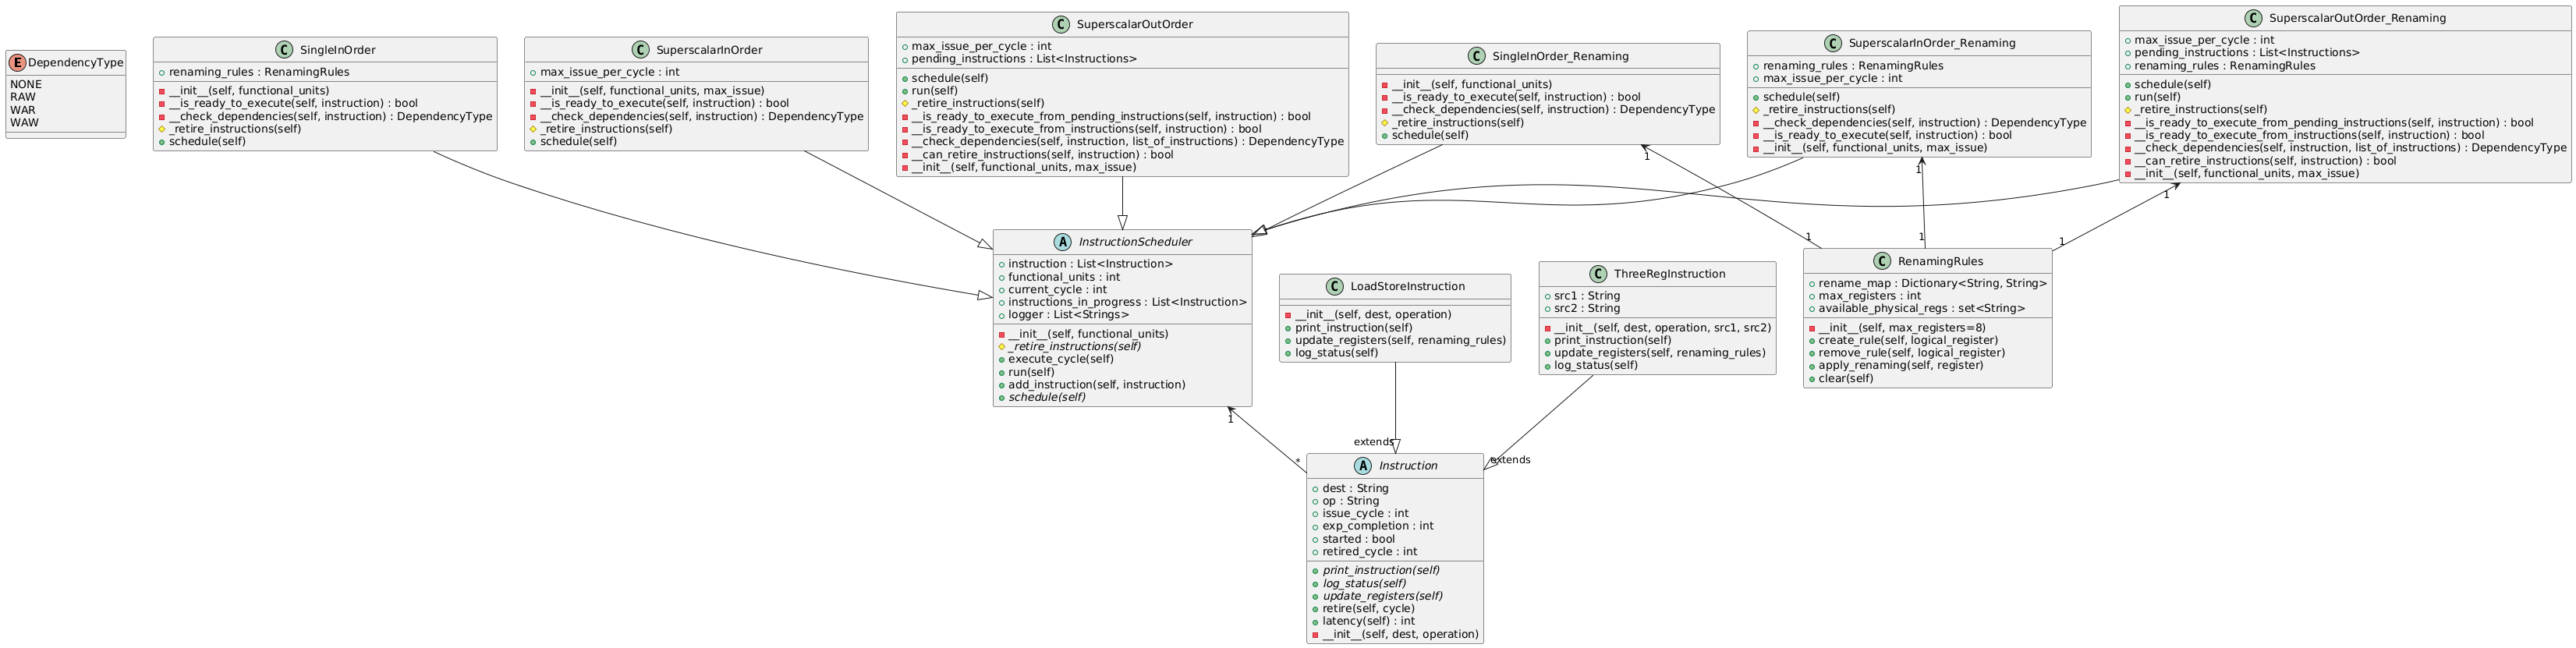
\includegraphics[width=1\textwidth]{ClassDiagram.png}  
    \caption{Class Diagram of Design, developed using the Plant UML tools.}  
    \label{fig:ClassDiagram}
\end{figure}
The diagram in figure \ref{fig:ClassDiagram} encapsulates the logic that helped develop this simulation. In the following subsections, I will be explaining the logic and reasons behind each class seen in here.

\subsection{Instruction Scheduler Abstract Class}
The instruction scheduler was the layout all configurations should have, and contained the overlapping logic. It looked to highlight possibly repeated concrete methods and abstract methods, that each subclass should implement. The properties contained here where the following:
\begin{itemize}
    \item \lstinline|instructions|: instructions that should be executed by the scheduler
    \item \lstinline|functional_units|: the number of parallel functional units in the scheduler
    \item \lstinline|current_cycle|: the value of the current cycle
    \item \lstinline|instructions_in_progress|: instructions that are currently in functional units
    \item \lstinline|logger|: a list of strings, that where used to log results and debug statements
\end{itemize}

All schedulers contained these properties, and additional properties came when we introduced register renaming or out of order execution and retirement. Now, let's look at the methods defined for this hierarchy. 
\begin{itemize}
    \item \lstinline|__init__(self, functional_units)|: this function is helps the creation of instruction scheduler's instances. Filling up overlapping properties, when creating an instance.
    \item \lstinline|run(self)|: the logic for running is the same for nearly all schedulers. This method is in charge of executing cycles until all instructions have been dispatched out of the scheduler. 
    \item \lstinline|add_instruction(self, instruction)|: this method is in charge of dynamically adding an instruction to the list of instructions of a scheduler.
    \item \textit{\lstinline|_retire_instructions(self)|}: this method is abstract since depending on the type of configuration of an instruction scheduler, different retirement logic should be implemented. Thus, this method is in charge of indicating that each subclass should define instruction retirement.
    \item \textit{\lstinline|schedule(self)|}: this method is also abstract since it should define the main logic of instruction scheduling which is dependent on the configuration type.
\end{itemize}


\section{Methodology}

\section{Tests}

\section{Results}

\section{Discussion}

\end{document}